\chapter{解的存在唯一性}
本章旨在确定形如
\[
\frac{d\bm{x}}{dt}=f(t,\bm{x}),\quad \bm{x}(t_0)=\bm{x}^0
\]
的初值问题什么时候存在唯一解。由于教材中只介绍了存在唯一性定理，而对
解的延拓提之甚少，而仅在小范围有解对我们判断方程的解帮助不大，故本章摒
弃教材内容，采用《常微分方程定性与稳定性方法》一书的讲解方法。

\section{存在唯一性定理}\label{sec:1.1}
首先给出存在唯一性定理。
\begin{thm}[(存在唯一性定理)]\label{thm:1.1.1}
考虑初值问题（又称 Cauchy 问题）:
\begin{equation}\label{equ:1.1}
    \left\{
        \begin{aligned}
            &\frac{d\bm{x}}{dt}=\bm{f}(t,\bm{x}),\\
            &\bm{x}(t_0)=\bm{x}^0,
        \end{aligned}
    \right.
\end{equation}
其中 $\bm{x}\in\R^n, f:\R\times\R^n\to\R^n$. 若 $\bm{f}(t,\bm{x})$ 在开区域 $G\subset\R\times\R^n$中满足：
\begin{description}
    \item[(i)] $\bm{f}\in C(G)$;
    \item[(ii)] $\bm{f}$ 关于 $\bm{x}$ 满足局部 Lipschitz 条件，即对于点 $P_0(t_0,\bm{x}^0)\in G$, 存在
    \[
    G_0=\{[t,\bm{x}]:|t-t_0|\leq a,\|\bm{x}-\bm{x}^0\|\leq b\}\subset G,
    \]
    和依赖于 $P_0$ 的常数 $L_{P_0}$, 使得 $\forall (t,\bm{x}^1),(t,\bm{x}^2)\in G_0$，有不等式
    \begin{equation}\label{equ:1.2}
        \|\bm{f}(t,\bm{x}^1)-\bm{f}(t,\bm{x}^2)\|\leq L_{P_0}\|\bm{x}^1-\bm{x}^2\|.
    \end{equation}
    成立，其中 $\|\cdot\|$ 表示欧式范数.
\end{description}

则 Cauchy 问题 (\ref{equ:1.1}) 在区间 $|t-t_0|\leq h^*$ 上存在唯一解，其中
\[
0<h^*<\min\{h,\frac{1}{L_{P_0}}\},\quad h=\min\{a,\frac{b}{M}\},\quad M=\max_{(t,\bm{x})\in G_0}\|f(t,\bm{x})\|.
\]
\end{thm}

\begin{pf1}
容易证明式 (\ref{equ:1.1}) 等价于
\begin{equation}\label{equ:1.3}
    \bm{x}(t)=\bm{x}^0+\int_{t_0}^tf(\tau,\bm{x}(\tau))d\tau.
\end{equation}
取 $B$ 为定义在区间 $|t-t_0|\leq h^*$ 上的连续函数所构成的空间，$D$
为定义在区间 $|t-t_0|\leq h^*$ 上且图像包含 $G_0$ 的所有连续函数构
成的集合. 现定义在 $C(B)$ 上的映射
\begin{equation}\label{equ:1.4}
    (T\bm{x})(t)=\bm{x}^0+\int_{t_0}^tf(\tau,\bm{x}(\tau))d\tau,\quad |t-t_0|\leq h^*.
\end{equation}
由于
\[
\|T\bm{x}-\bm{x}^0\|\leq\left|\int_{t_0}^t\|f(\tau,\bm{x}(\tau))\|d\tau\right|\leq M|t-t_0|\leq b,
\]
故映射 (\ref{equ:1.4}) 把集合 $D$ 映射到自身. 

任取 $\bm{x}^1,\bm{x}^2\in D$, 由于
\[
\begin{array}{rl}
    \|T\bm{x}^1-T\bm{x}^2\|_C&=\max\limits_{|t-t_0|\leq h^*}\|\int_{t_0}^{t}\left[f(\tau,\bm{x}^1(\tau))-f(\tau,\bm{x}^2(\tau))\right]d\tau\|\\
    & \leq \max\limits_{|t-t_0|\leq h^*}\left|\int_{t_0}^t\|f(\tau,\bm{x}^1)-f(\tau,\bm{x}^2)\|d\tau\right|\\
    & \leq L_{P_0}h^*\|\bm{x}^1-\bm{x}^2\|_C.
\end{array}
\]
且 $L_{P_0}h^*<1$，根据压缩映射原理，映射 (\ref{equ:1.4}) 存在唯一不
动点，即在区间 $|t-t_0|\leq h^*$ 上 (\ref{equ:1.3}) 存在唯一解，于是定理
\ref{thm:1.1.1} 证毕.
\end{pf1}

若将定理 \ref{thm:1.1.1} 中的因变量 $\bm{x}$ 降为一维 $x$，则该定理
类似于教材中的唯一分解定理。虽然 Picard 迭代书写证明相较于压缩映射更
为复杂，但这个证明思路确是不得不品的一环。

下面给出一维存在唯一性定理及 Picard 迭代证明.
\begin{thm}[(存在唯一性定理)]\label{thm:1.1.2}
考虑 Cauchy 问题：
\begin{equation}\label{equ:1.5}
\left\{
\begin{aligned}
& \frac{dy}{dx} = f(x,y), \\
& y(x_0) = y_0
\end{aligned}
\right.
\end{equation}
其中 \(f(x,y)\) 在矩形区域 $R=\{(x,y): |x - x_0| \le a, |y - y_0| \le b\},$
上连续，并且对 \(y\) 满足Lipschitz 条件, 即存在 \(L > 0\), 使对所有 \((x, y_1), (x, y_2) \in R\) 成立
\begin{equation*}
|f(x, y_1) - f(x, y_2)| \le L |y_1 - y_2|
\end{equation*}
则初值问题(\ref{equ:1.5})在区间 \(|x - x_0| \le h\) 上的解存在且唯一，其中 \(h = \min(a, \frac{b}{M}), M = \max\limits_{(x,y) \in R} |f(x,y)|\)
\end{thm}
\begin{pf1}
先证明存在性。首先，容易验证式 (\ref{equ:1.5}) 等价于
\begin{equation}\label{equ:1.6}
y(x)=y_0+\int_{x_0}^xf(s,y(s))ds.
\end{equation}
考虑如下函数列：
\begin{equation}\label{equ:1.7}
\varphi_0(x)=y_0,\quad \varphi_n(x)=y_0+\int_{x_0}^xf(s,\varphi_{n-1}(s))ds,\quad n\geq 1. 
\end{equation}
由于
\[
|\varphi_n(x)-y_0|\leq\left|\int_{x_0}^{x}|f(s,\varphi(s))|ds \right|\leq M|x-x_0|\leq b,
\]
因此 (\ref{equ:1.7}) 中的函数都落在 $R$ 中。接着，我们断言
\begin{equation}\label{equ:1.8}
|\varphi_n(x)-\varphi_{n-1}(x)|\leq\frac{ML^{n-1}}{n!}|x-x_0|^n.
\end{equation}
采用数学归纳法，当 $n=1$ 时有
\[
|\varphi_1(x)-\varphi_0(x)|=\left|\int_{x_0}^xf(s,y_0)ds\right|\leq M|x-x_0|,
\]
此时式 (\ref{equ:1.8}) 显然成立.假设 $n$ 时式 (\ref{equ:1.8}) 成立，则
\begin{align*}
|\varphi_{n+1}(x)-\varphi_n(x)|
  &\le \left|\int_{x_0}^x |f(s,\varphi_n(s))-f(s,\varphi_{n-1}(s))|\,ds\right|\\
  &\le L\left|\int_{x_0}^x |\varphi_n(s)-\varphi_{n-1}(s)|\,ds\right|\\
  &\le \frac{ML^n}{n!}\left|\int_{x_0}^x |s-x_0|\,ds\right|\\
  &= \frac{ML^n}{n!}\cdot\frac{1}{n+1}|x-x_0|^{n+1}.
\end{align*}
因此式 (\ref{equ:1.8}) 对任意 $n$ 都成立.

然后，由于 $\{\varphi_n(x)\}$ 的一致收敛性与 $\sum_{k=1}^{n}\left(\varphi_k(x)-\varphi_{k-1}(x)\right)$ 的一致收敛性相等,
且
\[
\sum_{k=1}^n\left| \varphi_k(x)-\varphi_{k-1}(x) \right|\leq \sum_{k=1}^{n}\frac{ML^{k-1}}{k!}h^k\leq \frac{M}{L}e^{Lh}
\]
由 Weierstrass 判别法可知 $\{\varphi_n(x)\}$ 一致收敛，最后，记 $\varphi_n(x)\to \varphi(x)$，在 (\ref{equ:1.7}) 中令 $n\to\infty$ 有
\[
\varphi(x)=y_0+\lim_{n\to\infty}\int_{x_0}^{x}f(s,\varphi_n(s))ds=y_0+\int_{x_0}^{x}\lim_{n\to\infty}f(s,\varphi_n(s))ds=y_0+\int_{x_0}^{x}f(s,\varphi(s))ds,
\]
因此 $\varphi(x)$ 是 (\ref{equ:1.5}) 的解，存在性得证。

再证明唯一性。假设 $\varphi(x)$ 和 $\psi(x)$ 都是 (\ref{equ:1.6}) 的解，设 $h(x)=|\varphi(x)-\psi(x)|$,
则
\begin{equation}\label{equ:1.9}
h(x)\leq\int_{x_0}^x|f(s,\varphi(s))-f(s,\psi(s))|ds\leq L\int_{x_0}^xh(s)ds.
\end{equation}
再设 $H(x)=\int_{x_0}^xh(s)ds$, 则 $H'(x)=h(x)$，于是式 (\ref{equ:1.9}) 变为 $H'(x)-LH(x)\leq 0$, 乘上积分因子 $e^{-Lx}$ 可以得到
\[
(H(x)e^{-Lx})'\leq0
\]
由于 $H(x_0)=0$, 因此对 $\forall x>x_0, H(x)e^{-Lx}\leq0, H(x)\leq 0$. 但是由于 $h(x)\geq0,$ 当 $x>x_0$ 时，$H(x)\geq0$，
因此 $H(x)\equiv 0,\forall x>x_0$. $x<x_0$ 的情况同理. 最终，$\varphi(x)\equiv\psi(x)$, 唯一性得证.
\end{pf1}

\begin{figure}[htbp]
    \centering
    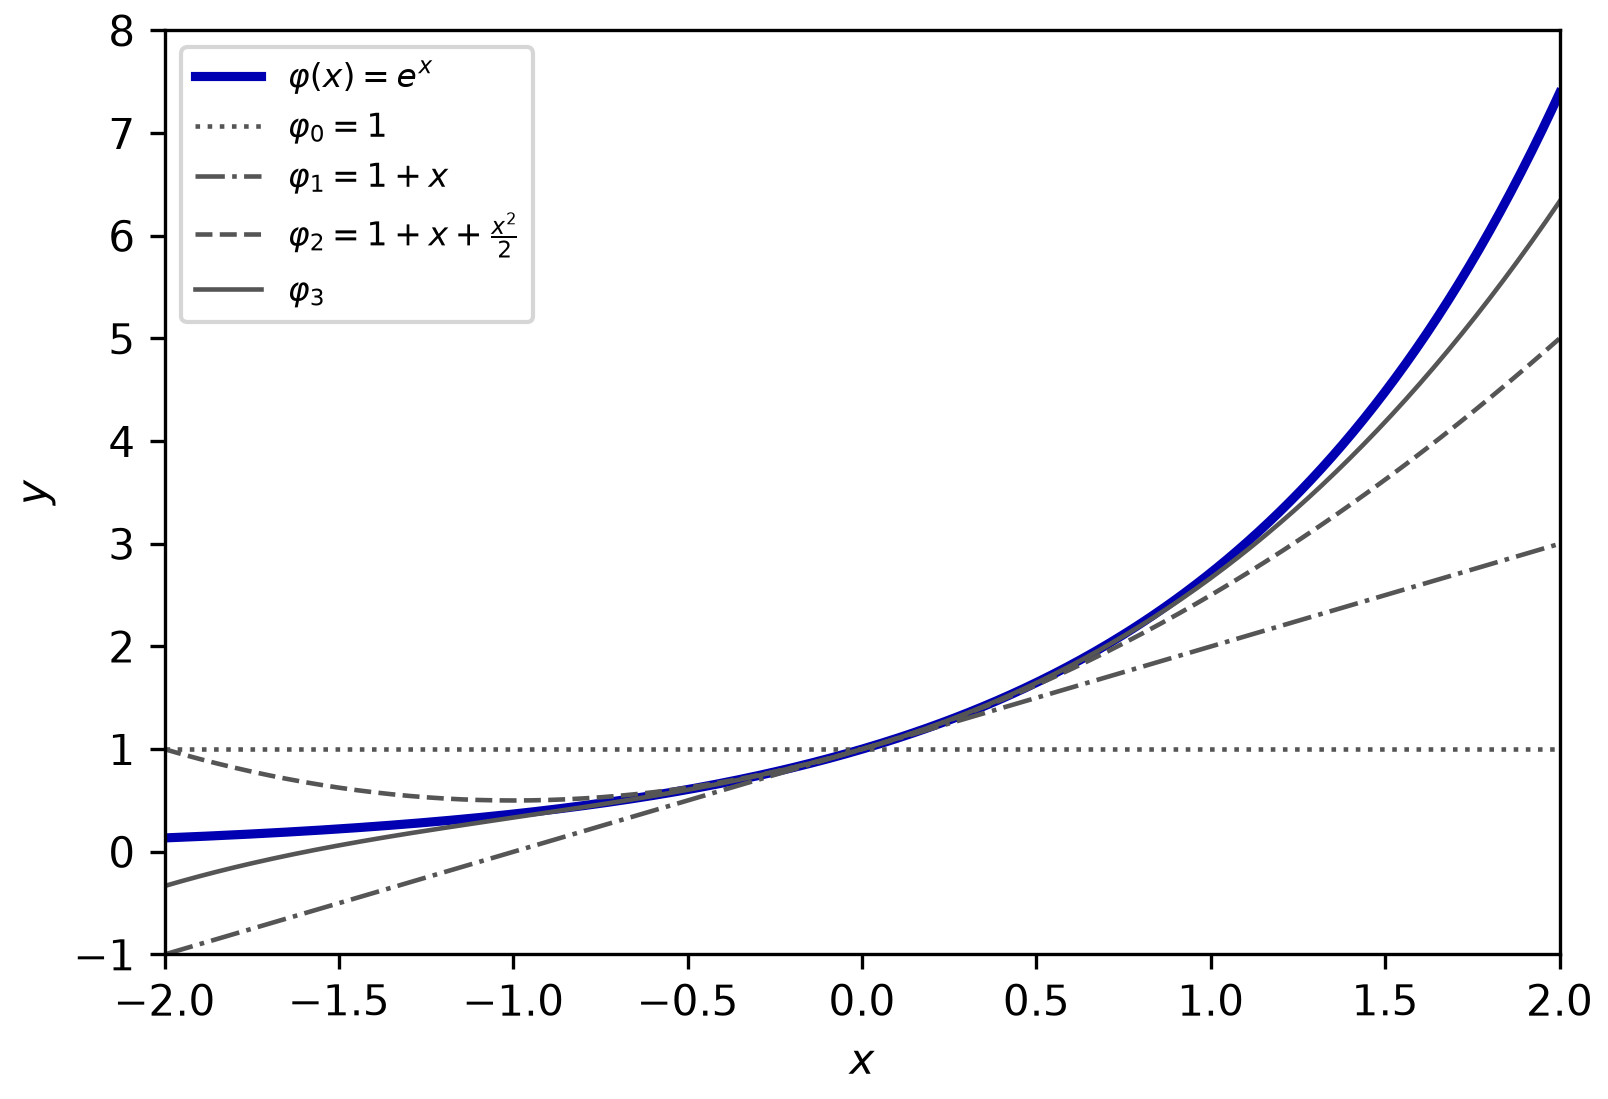
\includegraphics[width=0.6\linewidth]{pic/fig1.1_picard.png}
    \caption{方程 $y'=y,\ y(0)=1$ 的 Picard 迭代序列 $\varphi_n(x)$ 对解
    $\varphi(x)=e^x$ 的逼近}
\end{figure}

\begin{rmk}
\begin{description}
\item[(i)] 应当指出，无论是定理 \ref{thm:1.1.1} 还是定理 \ref{thm:1.1.2}, 
仅有 $\bm{f}$ 的连续性条件就足以保证解的存在性，
Lipschitz 条件保证解至多只有一个，却不保证其存在性.
且这两个条件都只是充分条件而非必要条件.
\item[(ii)] 注意到，定理 \ref{thm:1.1.1} 相比于 定理 \ref{thm:1.1.2},其所确定的
存在唯一区间更小，这是所用方法导致的. 但是在下一讲研究了解的延拓之后，
局部区间的大小便显得无关紧要了.
\end{description}
\end{rmk}


\section{解的延拓}\label{sec:1.2}
当对 (\ref{equ:1.1}) 初值问题进行一次存在唯一性定理，可以得到一个存在唯一区间
$[t_0-h^*,t_0+h^*]$. 此时我们发现在该区间的边界还可以再次使用存在唯一定理，
于是解的存在区间扩大了，这就是对解进行延拓的思想.当我们反复进行如上操作，
理论上会得到一个存在区间，称为\textbf{解的最大存在区间}. 显然该区间
必为包含 $t_0$ 开区间，否则可以继续延拓, 记为 $(\alpha, \beta)$. 于是
我们接下来的目标就是求出 $(\alpha,\bm{x}(\alpha))$ 和 $(\beta,\bm{x}(\beta))$
在哪.

\begin{figure}[H]
    \centering
    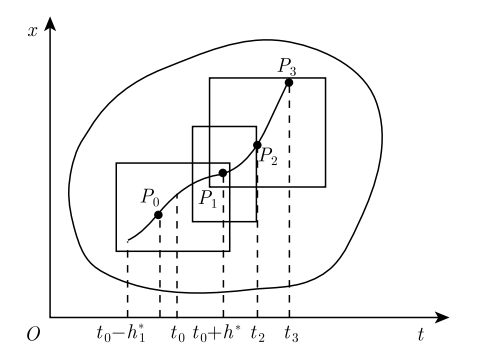
\includegraphics[width=0.5\linewidth]{pic/fig1.2_extension.png}
    \caption{解的延拓}
\end{figure}

\begin{thm}\label{thm:1.2.1}
设 $\bm{f}(t,\bm{x})$ 在域 $G\subset \R\times\R^n$ 内连续有界，且对 $\bm{x}$
满足局部 Lipschitz 条件，若 Cauchy 问题 (\ref{equ:1.1}) 的解 $\bm{x}(t)$
的最大存在区间为 $(\alpha,\beta), \alpha,\beta$ 为有限数，则
\begin{description}
    \item[(i)] 极限 $\lim_{t\to\alpha^+}\bm{x}(t)=\bm{x}(\alpha^+)$ 和 $\lim_{t\to\beta^-}\bm{x}(t)=\bm{x}(\beta^-)$ 存在；
    \item[(ii)] 点 $(\alpha,\bm{x}(\alpha^+))$ 和 $(\beta,\bm{x}(\beta^-))$ 均在 $G$ 的边界上.
\end{description}
\end{thm}
\begin{pf1}
\textbf{(i)} 由 Cauchy 问题 (\ref{equ:1.1}) 的等价积分方程
\[
\bm{x}(t)=\bm{x}^0+\int_{t_0}^tf(\tau,\bm{x}(\tau))d\tau.
\]
可知，
\[
\begin{aligned}
\|\boldsymbol{x}(t_1)-\boldsymbol{x}(t_2)\|
&= \left\| \int_{t_0}^{t_1} \boldsymbol{f}(\tau,\boldsymbol{x}(\tau))\mathrm{d}\tau
- \int_{t_0}^{t_2} \boldsymbol{f}(\tau,\boldsymbol{x}(\tau))\mathrm{d}\tau \right\| \\
&= \left\| \int_{t_2}^{t_1} \boldsymbol{f}(\tau,\boldsymbol{x}(\tau))\mathrm{d}\tau \right\| \\
&\leqslant \left| \int_{t_2}^{t_1} \|\boldsymbol{f}(\tau,\boldsymbol{x}(\tau))\| \mathrm{d}\tau \right|
\leq M|t_1-t_2|,
\end{aligned}
\]
其中 $M$ 为 $\|\boldsymbol{f}(t,\boldsymbol{x})\|$ 的上界。

由于 $\beta$ 为有限数, 所以, 当 $t_1,t_2 \to \beta^-$ 时, 有 $\|\boldsymbol{x}(t_1)-\boldsymbol{x}(t_2)\| \to 0$。由 Cauchy 收敛准则得知极限 $\boldsymbol{x}(\beta-0)$ 存在。同理可证 $\boldsymbol{x}(\alpha+0)$ 存在。

\textbf{(ii)} 若它们不在边界上，则它们就是 $G$ 的内点，于是可继续延拓，这与 $(\alpha,\beta)$ 为最大存在区间矛盾.
\end{pf1}

若去掉 $\bm{f}$ 有界的假设，则可得到如下定理.
\begin{thm}\label{thm:1.2.2}
设 $\bm{f}(t,\bm{x})\in C(G\subset\R\times\R^n)$，且对 $\bm{x}$ 满足局部 Lipschitz 条件，
则 Cauchy 问题 (\ref{equ:1.1}) 的解可延拓到与 $G$ 的边界任意接近（包括可能趋于无穷）. 
\end{thm}
\begin{pf1}
作有界区域 $G_n(n=1,2,\cdots)$，满足 $(t_0,\bm{x}^0)\in G_1\subset G_2\subset \cdots\subset G, \overline{G}_n\subset G_{n+1}, G_n\to G$.
由于 $\bm{f}$ 在 $\overline{G}_n$ 内有界，根据定理\ref{thm:1.2.1} 可
延拓到 $\overline{G}_n$ 的某一边界点 $P_n$，这样得到点列 $\{P_n\}$.
由于 $G_n\to G$，故 $\{P_n\}$ 可以与 $G$ 任意接近.
\end{pf1}
\begin{rmk}
虽然该解可延拓到与 $G$ 任意接近，但是不意味可以趋于边界上的某个点，因为 $\{P_n\}$ 不一定收敛.
\end{rmk}

注意到，若 $G$ 为全空间 $\R\times\R^n$，则定理 \ref{thm:1.2.1} 中的
最大存在区间 $(\alpha,\beta)$ 就是 $\R$，但是定理 \ref{thm:1.2.2} 
中却不能这么保证，因为有可能在某一点 $t'$ 发生 $\lim_{t\to t'}\|\bm{x}(t)\|=\infty$,这种情况称为\textbf{在 $t'$ 点发生爆破}.
因此若 $\bm{f}$ 无界，为了防止爆破发生，必须有额外的限制条件.

\begin{figure}[htbp]
    \centering
    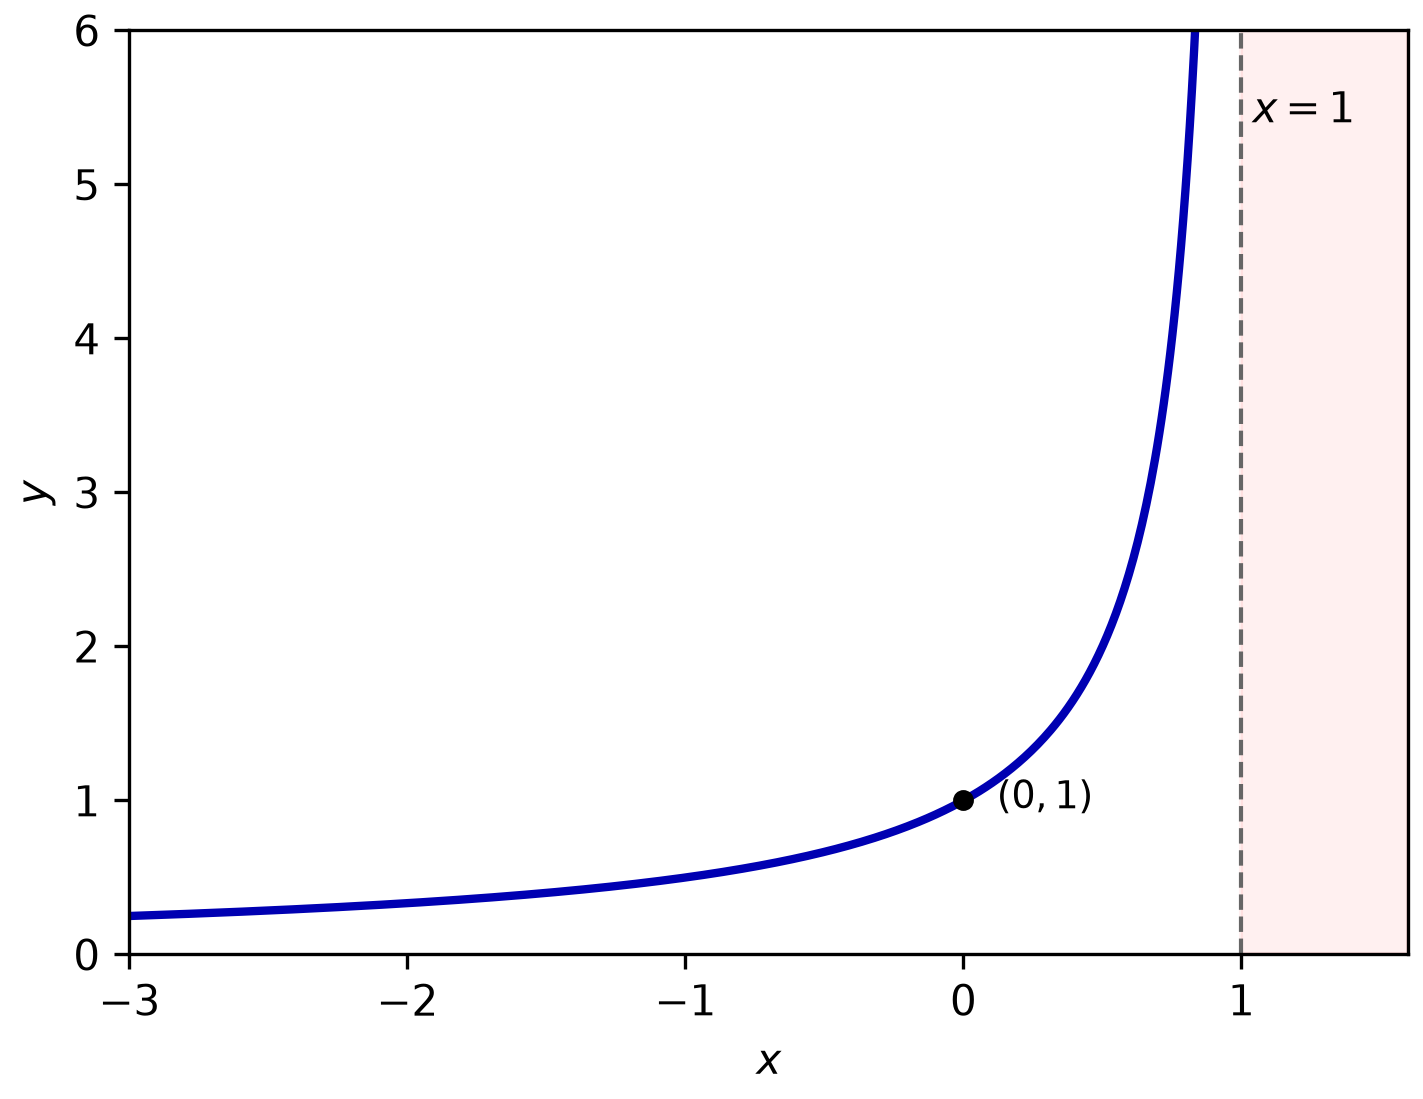
\includegraphics[width=0.5\linewidth]{pic/fig1.3_blowup.png}
    \caption{方程 $y'=y^2,\ y(0)=1$ 的解 $y=\dfrac{1}{1-x}$ 在 $x=1$ 处爆破，
    其最大存在区间为 $(-\infty,1)$}
\end{figure}

下面给出 $\bm{f}$ 有界的定理，以及 $\bm{f}$ 无界时的一种情况.
\begin{thm}\label{thm:1.2.3}
设 $\boldsymbol{f}(t,\boldsymbol{x})$ 在全空间 $\mathbb{R}\times\mathbb{R}^n$ 连续、有界，且对 $\boldsymbol{x}$ 满足局部Lipschitz条件，则 Cauchy 问题 (\ref{equ:1.1}) 解的存在区间为 $(-\infty,+\infty)$.
\end{thm}
\begin{thm}\label{thm:1.2.4}
设 $\boldsymbol{f}(t,\boldsymbol{x})$ 在全空间 $\mathbb{R}\times\mathbb{R}^n$ 连续，对 $\boldsymbol{x}$ 满足局部Lipschitz条件，且
\[
\|\boldsymbol{f}(t,\boldsymbol{x})\| \leqslant N\|\boldsymbol{x}\|,\quad N \text{ 为一正常数},
\]
则 $\forall\,(t_0,\boldsymbol{x}^0)\in\mathbb{R}\times\mathbb{R}^n$，Cauchy 问题 (\ref{equ:1.1}) 的解的存在区间均为 $(-\infty,+\infty)$。
\end{thm}

定理 \ref{thm:1.2.3} 的证明是容易的，请读者自证. 下面介绍定理 \ref{thm:1.2.4} 的证明，首先介绍一个著名的不等式.
\begin{lem}[(Gronwall)]\label{lem:1.2.1}
设 $C\geq 0, f(t),g(t\in C([a,b])), g(t)\geq 0$，且
\begin{equation}\label{equ:1.10}
f(t)\leq C+\int_{a}^tf(s)g(s)ds,\quad,a\leq t\leq b,
\end{equation}
则
\[
f(t)\leq C\exp\left(\int_a^tg(s)ds\right).
\]
\end{lem}
\begin{pf1}
设
\[
h(t)=C+\int_a^tf(s)g(s)ds,\quad a\leq t\leq b,
\]
则 $h(a)=C, h'(t)=f(t)g(t)$. 由 (\ref{equ:1.10}) 可知 $f(t)\leq h(t)$, 乘以 $g(t)$ 可得
\[
h'(t)-h(t)g(t)\leq 0,
\]
再乘以积分因子 $\exp\left(-\int_a^tg(s)ds\right)$，于是有
\[
\left(h(t)\exp\left(-\int_a^tg(s)ds\right)\right)'\leq0.
\]
结合 $h(a)\exp\left(-\int_a^ag(s)ds\right)=C$ 可知
\[
h(t)\exp\left(-\int_a^tg(s)ds\right)\leq C,
\]
于是
\[
f(t)\leq h(t)\leq C\exp\left(\int_a^tg(s)ds\right).
\]
\end{pf1}

下面证明定理 \ref{thm:1.2.4}.
\begin{pf1}
根据前面的分析，只需要证明对任意有界区间 $\bm{x}(t)$ 是有界，就可证明
解的存在区间为 $\R$.
由于
\begin{equation}\label{equ:1.11}
\|\bm{x}(t)\|\leq\|\bm{x}^0\|+\int_{t_0}^t\|\bm{f}(\tau,\bm{x}(\tau))d\tau\|\leq\|\bm{x}^0\|+\int_{t_0}^tN\|\bm{x}(\tau)d\tau\|,\forall t\geq t_0,
\end{equation}
根据 Gronwall 不等式，有
\[
\|\bm{x}(t)\|\leq\|\bm{x}^0\|\exp\left(\int_{t_0}^{t}Nd\tau\right)=\|\bm{x}^0\|e^{N(t-t_0)},\quad t\geq t_0.
\]
在 (\ref{equ:1.11}) 中令 $s=-\tau,y(t)=\|\bm{x}(-t)\|$ 可得
\[
\|\bm{x}(t)\|\leq\|\bm{x}^0\|e^{N(t_0-t)}
\]
因此对任意有界区间 $\bm{x}(t)$ 有界.
\end{pf1}
\begin{rmk}
从定理 \ref{thm:1.2.1} 到定理 \ref{thm:1.2.4}, 由于它们本质上都是使用存在唯一定理，因此最大存在区间在
保证了存在性的同时也保证了唯一性.
\end{rmk}

\section{比较定理}\label{sec:1.3}
由于比较定理不是本课程的重点，本节只做简单的定理介绍.

\begin{thm}[(第一比较定理)]
设有 Cauchy 问题
\[
(E_1)
\begin{cases}
    \dfrac{\mathrm{d}y}{\mathrm{d}x} = f(x, y), \\[10pt]
    y(x_0) = y_0,
\end{cases}
\qquad\qquad
(E_2)
\begin{cases}
    \dfrac{\mathrm{d}y}{\mathrm{d}x} = F(x, y), \\[10pt]
    y(x_0) = y_0,
\end{cases}
\]
其中 $f$ 和 $F$ 均在域 $G\subset \R\times\R$ 内连续且对 $y$ 满足
局部 Lipschitz 条件，$(x_0,y_0)\in G$，并设 $(E_1),(E_2)$ 的解均在
区间 $(a,b)$ 内连续. 若
\begin{equation}
f(x,y)<F(x,y),\quad\forall (x,y)\in G, 
\end{equation}
则
\begin{equation}
\begin{array}{c}
y(x)<Y(x),\quad x_0<x<b,\\
y(x)>Y(x),\quad a<x<x_0.
\end{array}
\end{equation}
\end{thm}
\begin{pf1}
令
\[
\varphi(x)=Y(x)-y(x),\quad x_0<x<b.
\]
由于 \(y(x)\) 与 \(Y(x)\) 分别是 \((E_1)\) 与 \((E_2)\) 的解，于是有
\begin{equation}\label{equ:1.14}
    \varphi'(x) = F(x, Y(x)) - f(x, y(x)),
\end{equation}
而且
\[
\begin{gathered}
    \varphi'(x_0) = F(x_0, y_0) - f(x_0, y_0) > 0, \\
    \varphi(x_0) = Y(x_0) - y(x_0) = 0.
\end{gathered}
\]
所以 \(\exists \delta > 0\)，使得
\begin{equation}\label{equ:1.15}
    \varphi(x) > 0, \quad x_0 < x < x_0 + \delta.
\end{equation}

以下证明不等式 (\ref{equ:1.15}) 在区间 \((x_0, b)\) 内成立. 假设不然，即至少有一点 \(\beta > x_0\)，\(\beta < b\)，使 \(\varphi(\beta) = 0\). 现把在 \((x_0, b)\) 内第一次使 \(\varphi(x) = 0\) 的 \(x\) 值记作 \(x_1\)，即
\[
    x_1 = \min\{x \mid \varphi(x) = 0, x_0 < x < b\},
\]
从而有
\[
    \varphi(x_1) = 0,
\]
即
\[
\begin{aligned}
    Y(x_1) &= y(x_1) \triangleq y_1, \\
    \varphi(x) &> 0, \quad x_0 < x < x_1.
\end{aligned}
\]
于是必有
\begin{equation}\label{equ:1.16}
    \varphi'(x_1) \leqslant 0.
\end{equation}
另一方面，由式 (\ref{equ:1.14}) 与定理条件可知
\[
\begin{aligned}
    \varphi'(x_1) &= F(x_1, Y(x_1)) - f(x_1, y(x_1)) \\
    &= F(x_1, y_1) - f(x_1, y_1) > 0,
\end{aligned}
\]
这与式 (\ref{equ:1.16}) 矛盾. 左行解同理. 定理得证.
\end{pf1}

\begin{figure}[H]
    \centering
    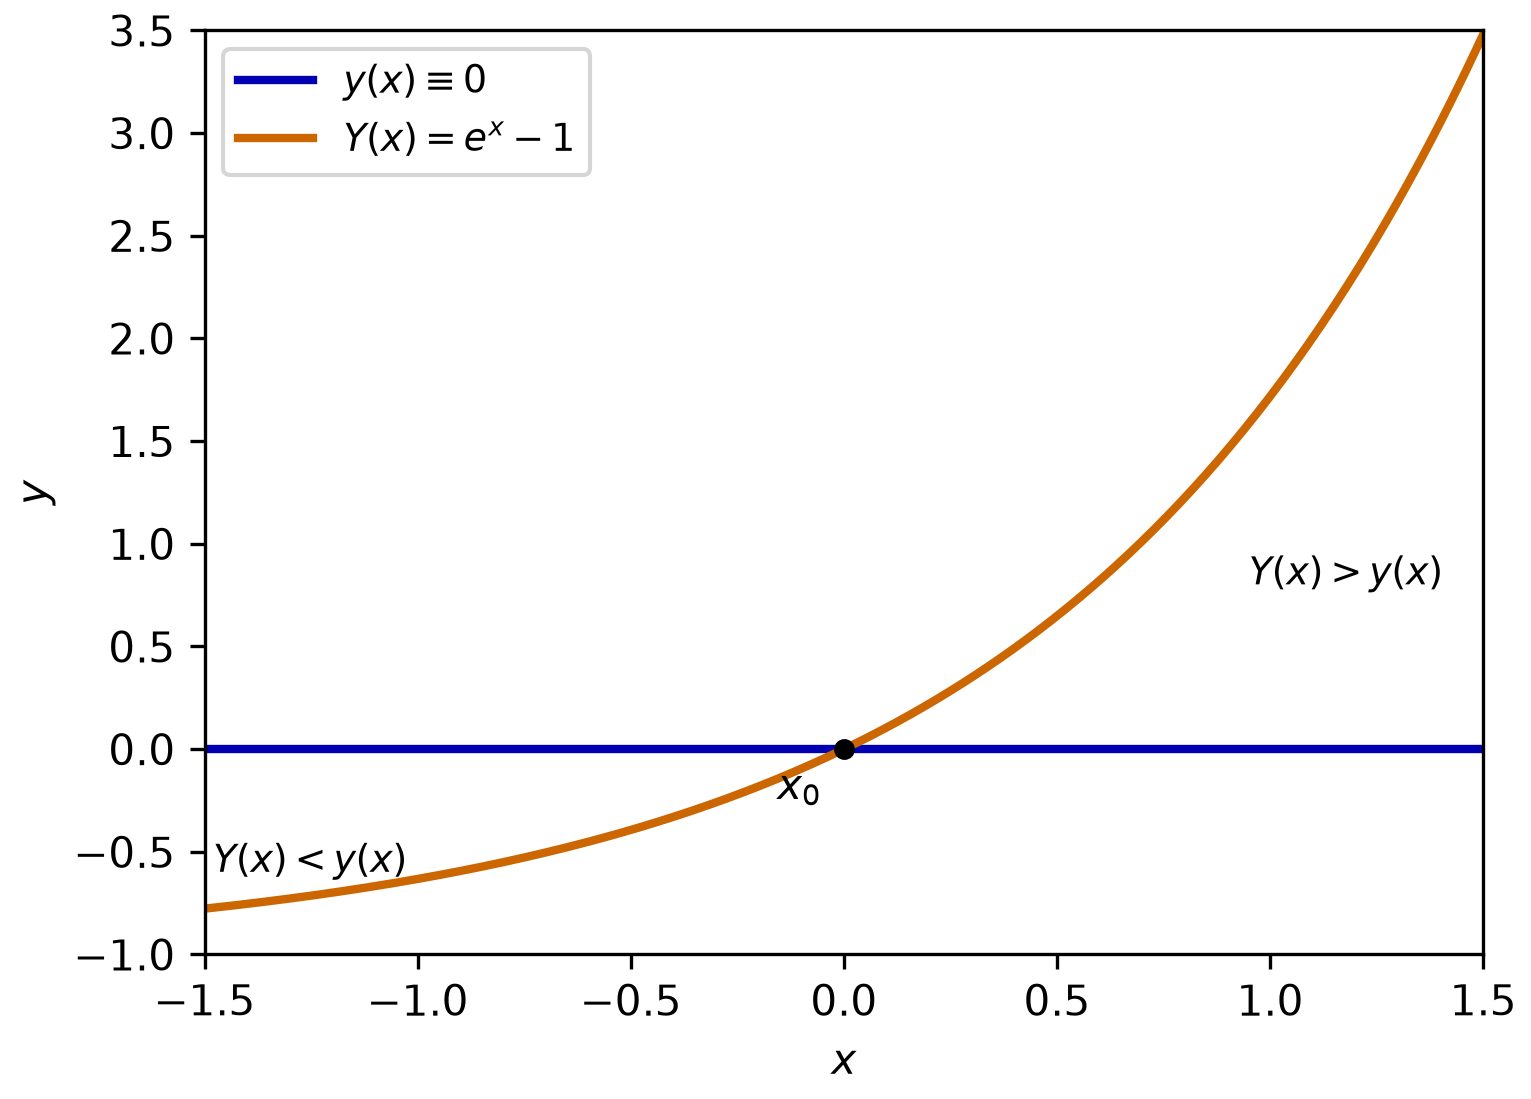
\includegraphics[width=0.5\linewidth]{pic/fig1.4_comparison.png}
    \caption{第一比较定理：$y'=y$ 的解 $y(x)\equiv0$ 与 $Y'=Y+1$ 的解
    $Y(x)=e^x-1$ 过同一点，$x>x_0$ 时 $Y(x)>y(x)$，$x<x_0$ 时 $Y(x)<y(x)$}
\end{figure}

\section{一阶微分方程的向量场}\label{sec:1.4}
前两节从分析的角度讨论了初值问题解的存在性与唯一性. 本节转向几何的角度：
不求解的具体表达式，而把右端函数在每一点的值看作该点处的一个方向，由此得到
向量场与积分曲线的几何图像. 这一观点不仅给出了求解的近似方法，而且构成了
定性理论的基础.

\subsection{向量场}\label{sec:1.4.1}
设一阶微分方程
\begin{equation}\label{equ:1.17}
\frac{dy}{dx}=f(x,y)
\end{equation}
的右端函数 $f(x,y)$ 在 $xy$ 平面的区域 $D$ 内有定义. 若 $f$ 在 $D$ 内连续且
关于 $y$ 满足局部 Lipschitz 条件，则由 \ref{sec:1.1} 节的存在唯一性定理，过
$D$ 内任一点
$(x_0,y_0)$，方程 (\ref{equ:1.17}) 有且仅有一个解 $y=\varphi(x)$ 满足
$\varphi(x_0)=y_0$. 从几何上看，解 $y=\varphi(x)$ 是 $xy$ 平面上的一条曲线，
称为方程 (\ref{equ:1.17}) 的\textbf{积分曲线}. 由
\[
\varphi'(x)=f(x,\varphi(x))
\]
可知，$f$ 在点 $(x,y)$ 处的值恰为过该点的积分曲线在该点处切线的斜率. 因此，
即使无法求出解的初等表达式，方程仍给出了 $D$ 内每一点处积分曲线切线方向的
信息.

\begin{deff}[(向量场)]
设 $f(x,y)$ 在区域 $D\subset\R^2$ 内有定义. 在 $D$ 内每一点 $(x,y)$ 处配置一个
以 $f(x,y)$ 为斜率的方向，等价地，配置非零向量
\[
\bm{v}(x,y)=(1,f(x,y)),
\]
由此在 $D$ 上得到的方向分布称为方程 (\ref{equ:1.17}) 所确定的\textbf{向量场}
（或\textbf{方向场}），$\bm{v}(x,y)$ 称为点 $(x,y)$ 处的\textbf{场向量}.
\end{deff}

形象地说，积分曲线就是始终沿着向量场的方向行进的曲线，它在每一点都与该点的
场向量相切. 于是，求方程 (\ref{equ:1.17}) 满足初值条件 $y(x_0)=y_0$ 的解，
等价于在向量场中寻找过点 $(x_0,y_0)$ 且处处与场向量相切的曲线. 这一几何事实
之所以重要，是因为当方程不可解时，可由向量场的走向近似地描绘积分曲线；更
重要的是，可以不经求解而由向量场的性质推断解的性质. 这正是近似解法与定性
理论的基本思想.

\begin{thm}\label{thm:1.4.1}
曲线 $L$ 为方程 (\ref{equ:1.17}) 的积分曲线的充要条件是：$L$ 上任一点处的
切线均与向量场在该点的场向量重合.
\end{thm}
\begin{pf1}
\textbf{必要性.} 设 $L$ 为方程 (\ref{equ:1.17}) 的积分曲线，其方程为
$y=\varphi(x)$，则 $\varphi$ 是 (\ref{equ:1.17}) 的解，于是在 $\varphi$ 的定义
区间上恒有
\[
\varphi'(x)=f(x,\varphi(x)).
\]
上式左端是 $L$ 在点 $(x,\varphi(x))$ 处切线的斜率，右端是向量场在同一点处场
向量的斜率，故二者方向重合. 由 $x$ 的任意性，$L$ 上每一点处均有此结论.

\textbf{充分性.} 设曲线 $L$ 的方程为 $y=\varphi(x)$，且在其上每一点
$(x,\varphi(x))$ 处，切线与场向量重合，则切线斜率与场向量的斜率相等，即
\[
\varphi'(x)=f(x,\varphi(x))
\]
在 $\varphi$ 的定义区间上恒成立. 这表明 $\varphi$ 是方程 (\ref{equ:1.17}) 的
解，从而 $L$ 为积分曲线.
\end{pf1}

\begin{rmk}
\begin{description}
\item[(i)] 定理 \ref{thm:1.4.1} 表明，积分曲线与向量场的关系是纯几何的，
与方程能否用初等函数求解无关. 求积分曲线，就是在向量场中作处处与场向量
相切的曲线.
\item[(ii)] 由存在唯一性定理，过 $D$ 内每一点恰有一条极大积分曲线，故积分
曲线族充满 $D$，且任意两条积分曲线在其公共存在区间上不相交. 换言之，
向量场的积分曲线构成了区域 $D$ 的一个不交覆盖.
\end{description}
\end{rmk}

\begin{figure}[htbp]
    \centering
    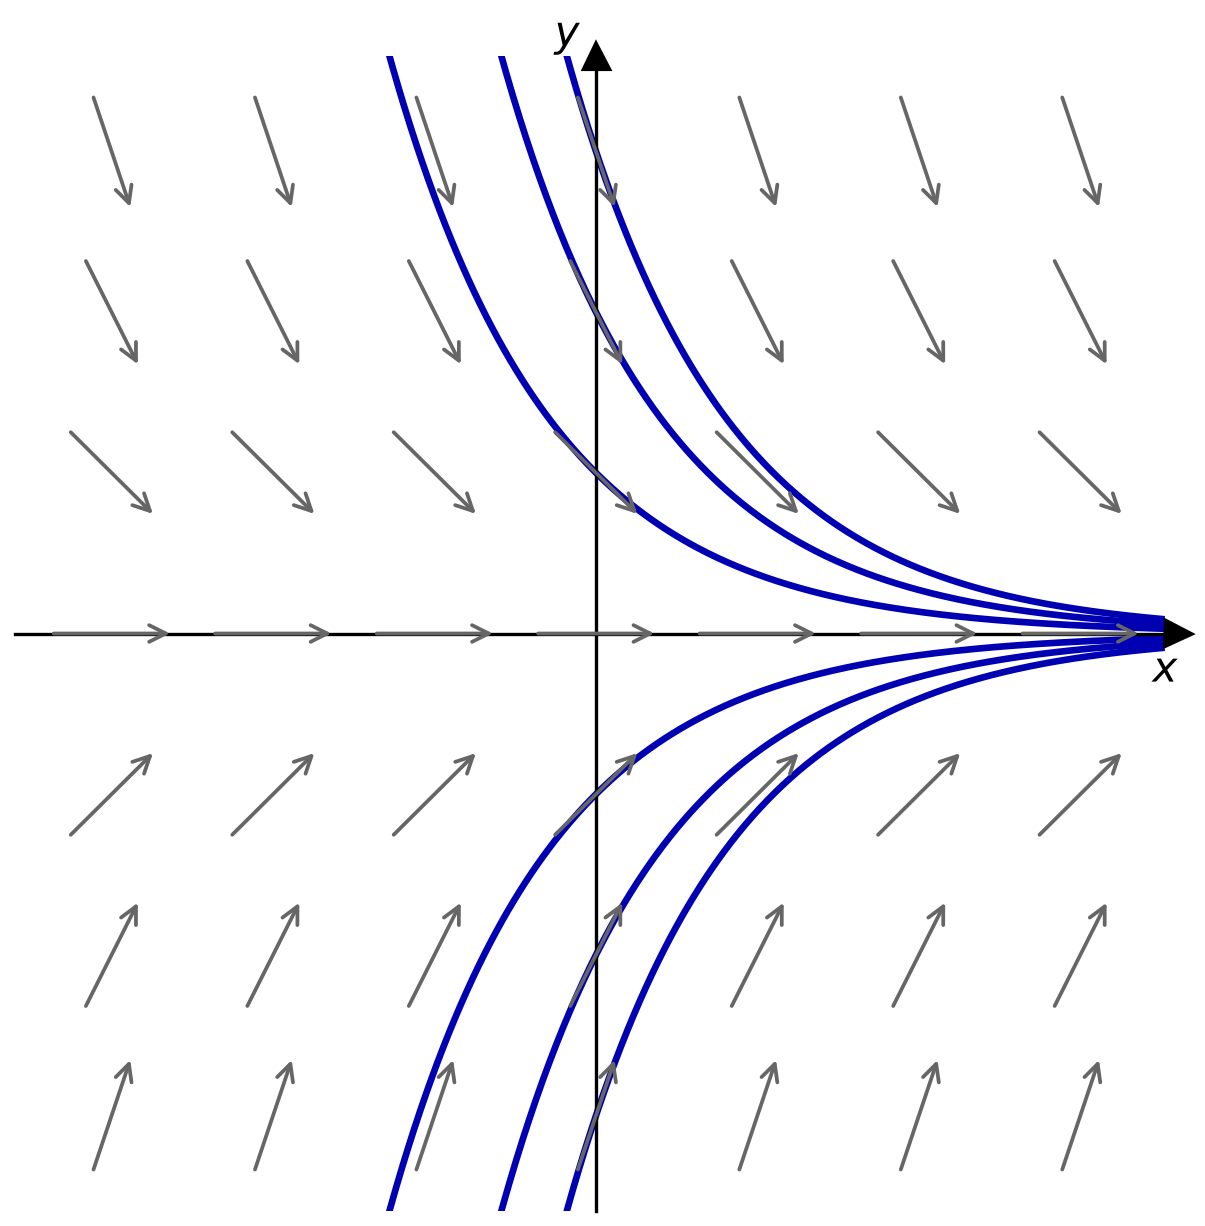
\includegraphics[width=0.5\linewidth]{pic/fig1.5_vectorfield.png}
    \caption{方程 $y'=-y$ 的向量场与积分曲线}
\end{figure}

\subsection{积分曲线的图解法}\label{sec:1.4.2}
图解法是不求出解的具体表达式，而直接根据右端函数的结构与向量场作出积分曲线
大致图形的方法. 它本质上是定性的，只能反映积分曲线的主要性态，却具有重要
的指导意义：能用初等方法求解的方程极少，而由向量场分析积分曲线的性态，
可以了解方程所刻画的实际现象的变化规律.

在 $D$ 内，场向量的斜率只依赖于 $f$ 在该点的值，因此 $f$ 取相同值的点处，
场向量互相平行，积分曲线的切线也互相平行. 利用这一特点可以大大减少绘制
向量场的工作量.

\begin{deff}[(等斜线)]
设 $c$ 为任意常数，称由方程
\begin{equation}\label{equ:1.18}
f(x,y)=c
\end{equation}
所确定的曲线为方程 (\ref{equ:1.17}) 的\textbf{等斜线}（又称\textbf{等倾线}）.
\end{deff}

等斜线 (\ref{equ:1.18}) 上每一点处场向量的斜率均为 $c$，故积分曲线在其上各点
的切线斜率均为 $c$. 于是，只需取若干常数 $c$，在相应的等斜线上画出斜率为
$c$ 的小线段，便得到向量场的大致图形. 例如，方程 $y'=-y$、$y'=x+y$、
$y'=x^2+y^2$ 的等斜线依次为 $y=-c$、$y=c-x$、$x^2+y^2=c$.

\begin{figure}[htbp]
    \centering
    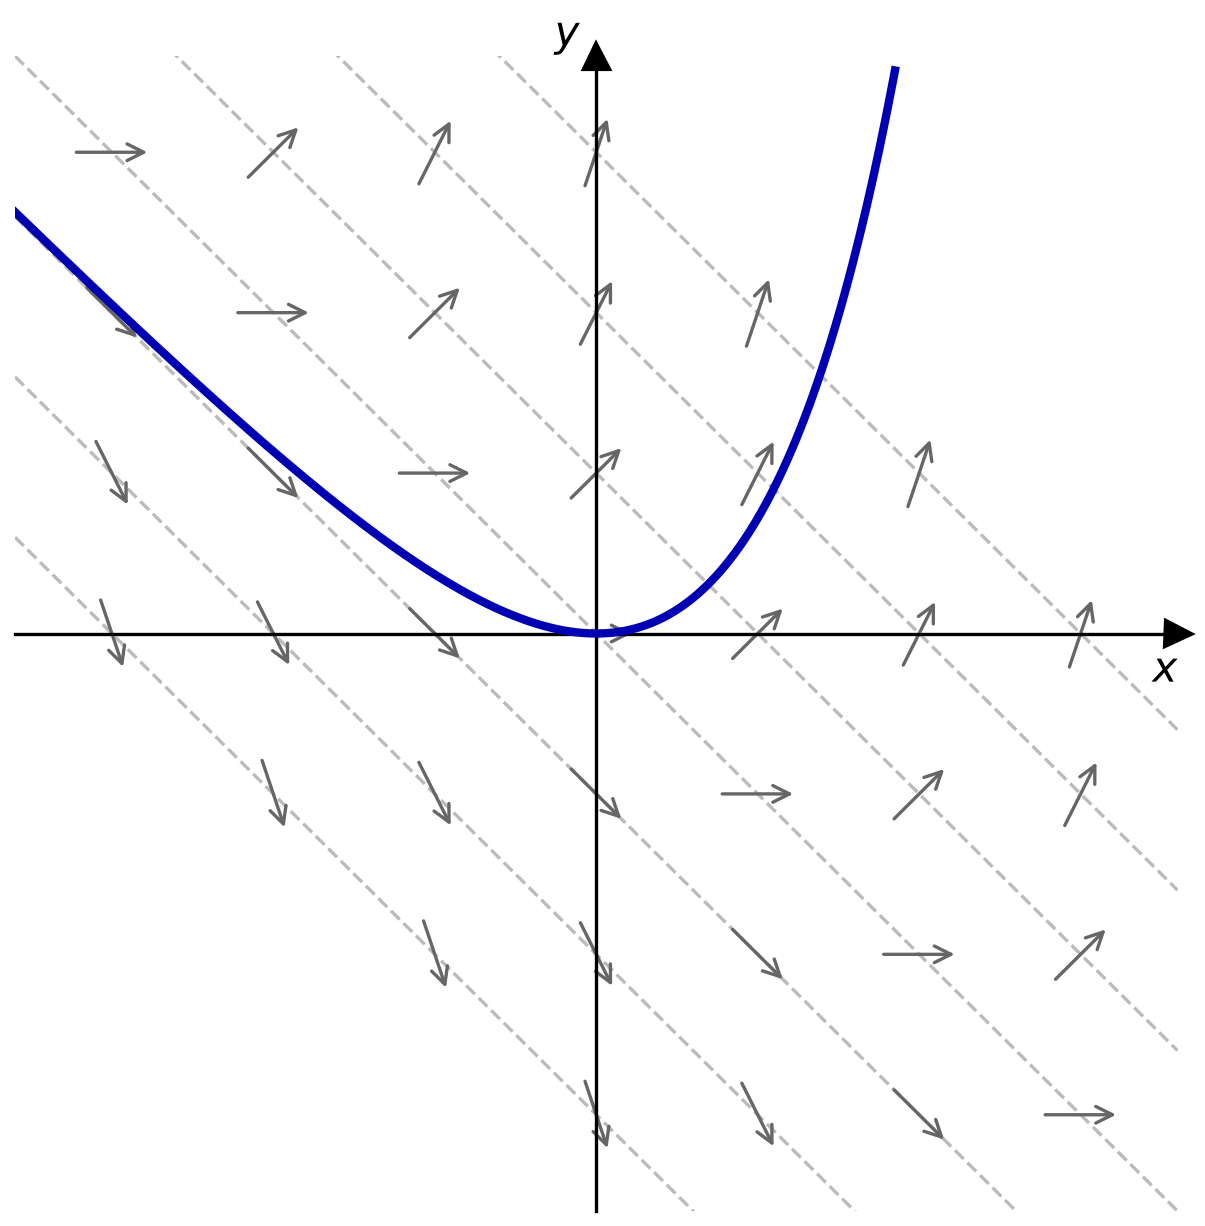
\includegraphics[width=0.5\linewidth]{pic/fig1.6_isocline.png}
    \caption{方程 $y'=x+y$ 的等斜线（虚线，$y=c-x$）与向量场；
    蓝线为过原点的积分曲线 $y=e^x-x-1$}
\end{figure}

在所有等斜线中，$c=0$ 的一条最为特殊. 称由
\[
f(x,y)=0
\]
确定的曲线为\textbf{零等斜线}. 在零等斜线上场向量的斜率为零，故积分曲线在
其上切线水平. 若零等斜线本身即为一条积分曲线，则它对应于一个常数解；否则，
积分曲线的极值只能在零等斜线上取得，因此零等斜线又称为\textbf{极值曲线}.

设 $f$ 有连续偏导数. 沿方程 (\ref{equ:1.17}) 的解求导，得
\begin{equation}\label{equ:1.19}
y''=f_x(x,y)+f_y(x,y)f(x,y).
\end{equation}
使 $y''=0$ 的点是积分曲线拐点的必要条件. 由
\[
f_x(x,y)+f_y(x,y)f(x,y)=0
\]
确定的曲线给出了积分曲线可能发生拐点的位置；若该曲线本身不是积分曲线，而
积分曲线在其上存在拐点，则称其为\textbf{拐点曲线}.

综上所述，用向量场作积分曲线的步骤可概括如下：
\begin{enumerate}
\item 取若干常数 $c$，画出等斜线 $f(x,y)=c$，并在其上标出斜率为 $c$ 的场
向量，得到向量场的骨架；
\item 画出零等斜线与拐点曲线，把区域 $D$ 分为若干部分，判定积分曲线在各部分
上的单调性与凹凸性；
\item 由存在唯一性定理确定解的存在区间，沿场向量的方向将相邻的场向量连成
光滑曲线，使其处处与场向量相切；
\item 结合 $y'$ 与 $y''$ 的符号以及极限性态，读出积分曲线的极值点、拐点与
渐近线.
\end{enumerate}

作为上述方法的补充，说明如何由右端函数判断积分曲线的渐近线. 设
$y=\varphi(x)$ 为一条积分曲线，若当 $x\to+\infty$ 时
$f(x,\varphi(x))\to k$，且 $\varphi(x)-kx$ 单调有界，则
$\varphi(x)-kx$ 有极限 $b$，于是该积分曲线以直线 $y=kx+b$ 为渐近线. 这说明
积分曲线在无穷远处的走向同样由 $f$ 在曲线附近的取值决定，无需解出
$\varphi$. 由此可见，向量场把微分方程的求解问题转化为几何作图问题，把解
的性态研究转化为向量场的结构研究，这正是定性理论的出发点.